
\noindent 

\includegraphics[width=4.5cm]{images/meshes/AMR/amr0}

\includegraphics[width=4.5cm]{images/meshes/AMR/amr1}
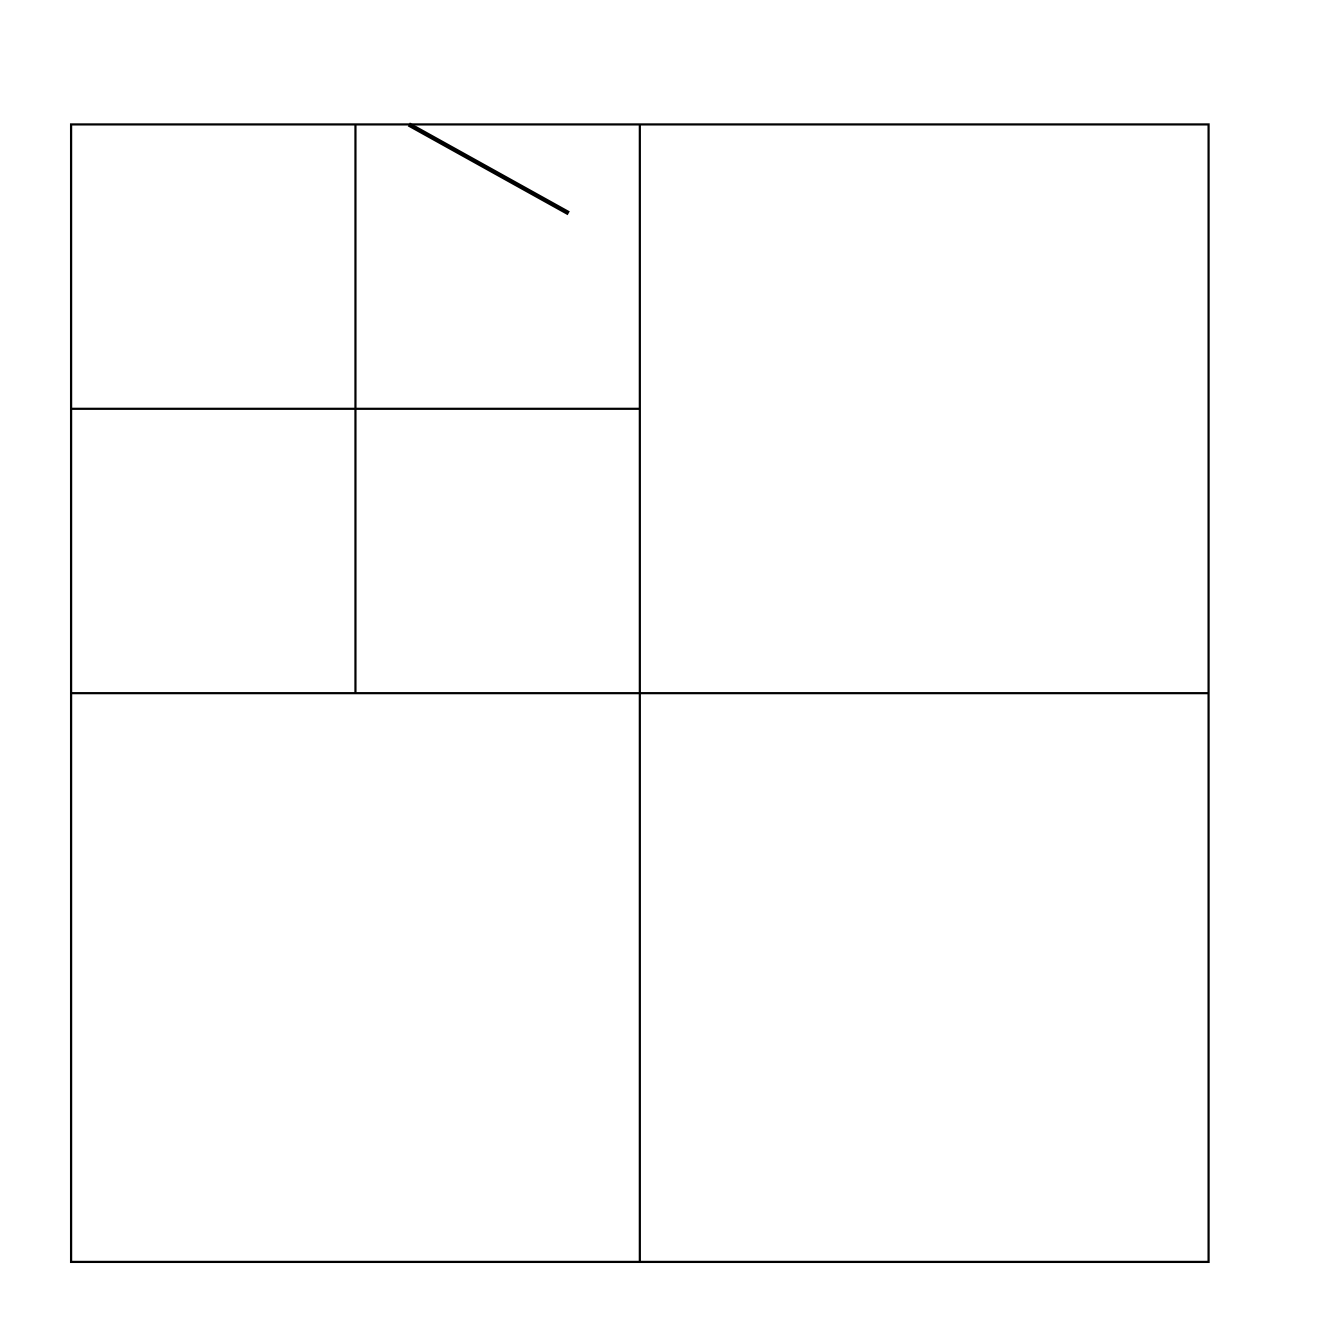
\includegraphics[width=4.5cm]{images/meshes/AMR/amr2}\\
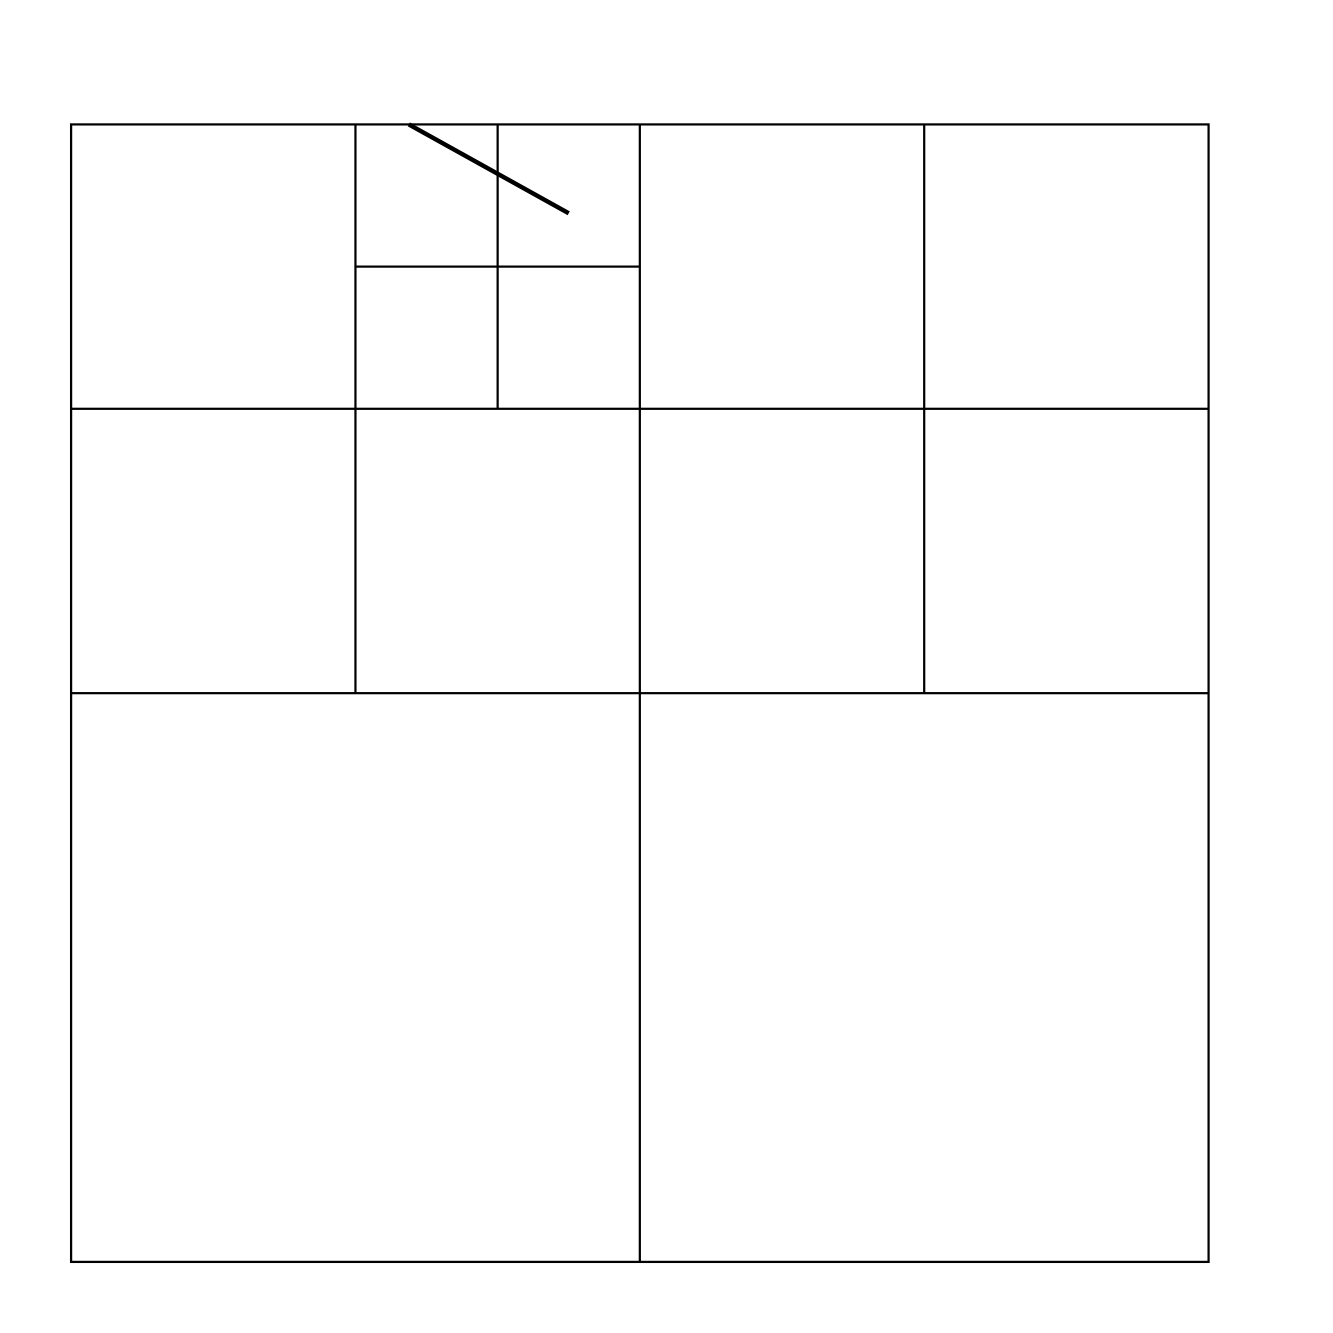
\includegraphics[width=4.5cm]{images/meshes/AMR/amr3}

\includegraphics[width=4.5cm]{images/meshes/AMR/amr4}

\includegraphics[width=4.5cm]{images/meshes/AMR/amr5}\\

\includegraphics[width=4.5cm]{images/meshes/AMR/amr6}

\includegraphics[width=4.5cm]{images/meshes/AMR/amr7}

\includegraphics[width=4.5cm]{images/meshes/AMR/amr8}

\begin{tabular}{l|ccccccccc}
             & \# l0  & \# l1 & \# l2 & \# l3 & \# l4 & \# l5 & \# l6 & \# l7 & \# l8 \\ 
\hline\hline
max level= 0 & 1 & \\
max level= 1 & 0 & 4 & \\
max level= 2 & 0 & 3 & 4 \\
max level= 3 & 0 & 2 & 7 & 4\\
max level= 4 & 0 & 2 & 5 & 10 & 8 \\
max level= 5 & 0 & 1 & 8 & 12 & 11 & 20 \\ 
max level= 6 & 0 & 1 & 8 & 11 & 13 & 20 & 32 \\
max level= 7 & 0 & 0 & 11 & 14 & 15 & 23 & 37 & 60 \\
max level= 8 & 0 & 0 & 11 & 13 & 17 & 27 & 43 & 72 & 116 \\
\hline
\end{tabular}

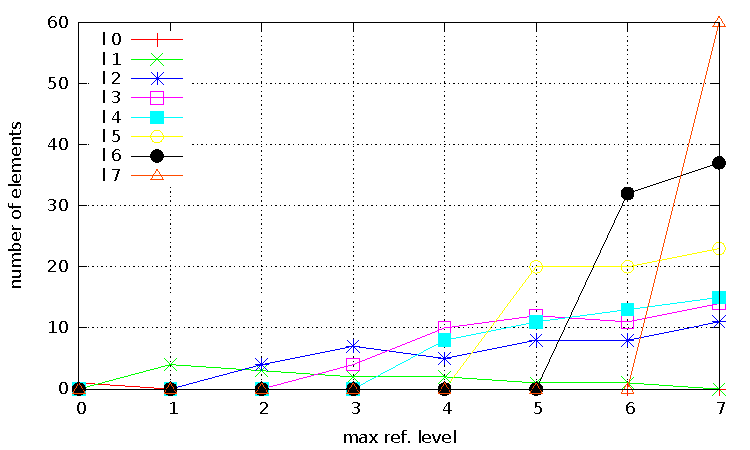
\includegraphics[width=7.28cm]{images/meshes/AMR/amr_data1.pdf}
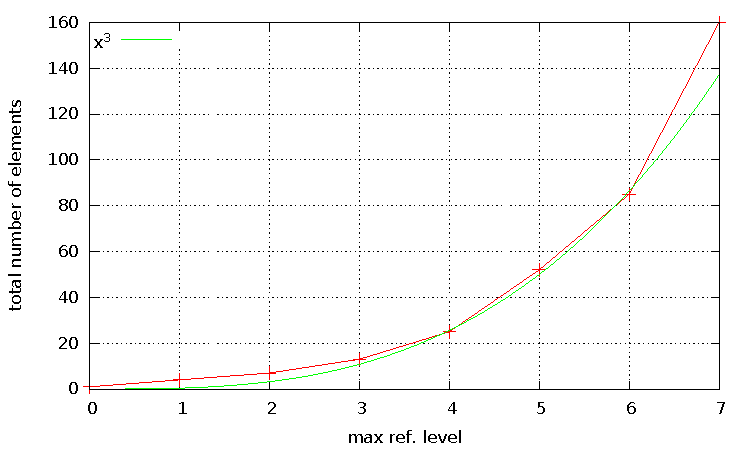
\includegraphics[width=7.28cm]{images/meshes/AMR/amr_data2.pdf}

In the particular case presented here, even though the inclusion in a short 
two-dimensional line, the total number of elements grows faster than the 
third power of the refinement level. While of course the total number 
of elements remains much smaller than the constant resolution counterpart, 
this observation tells us that authorising a unit increase of the maximum 
refinement level can have a substantial effect on the total number of elements.

\newpage

\noindent

\includegraphics[width=4cm]{images/meshes/AMR/amr_0}
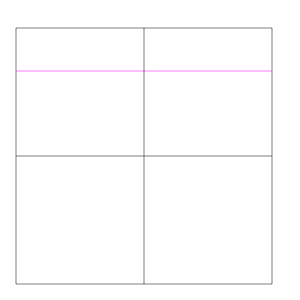
\includegraphics[width=4cm]{images/meshes/AMR/amr_1}
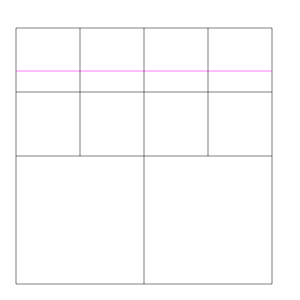
\includegraphics[width=4cm]{images/meshes/AMR/amr_2}
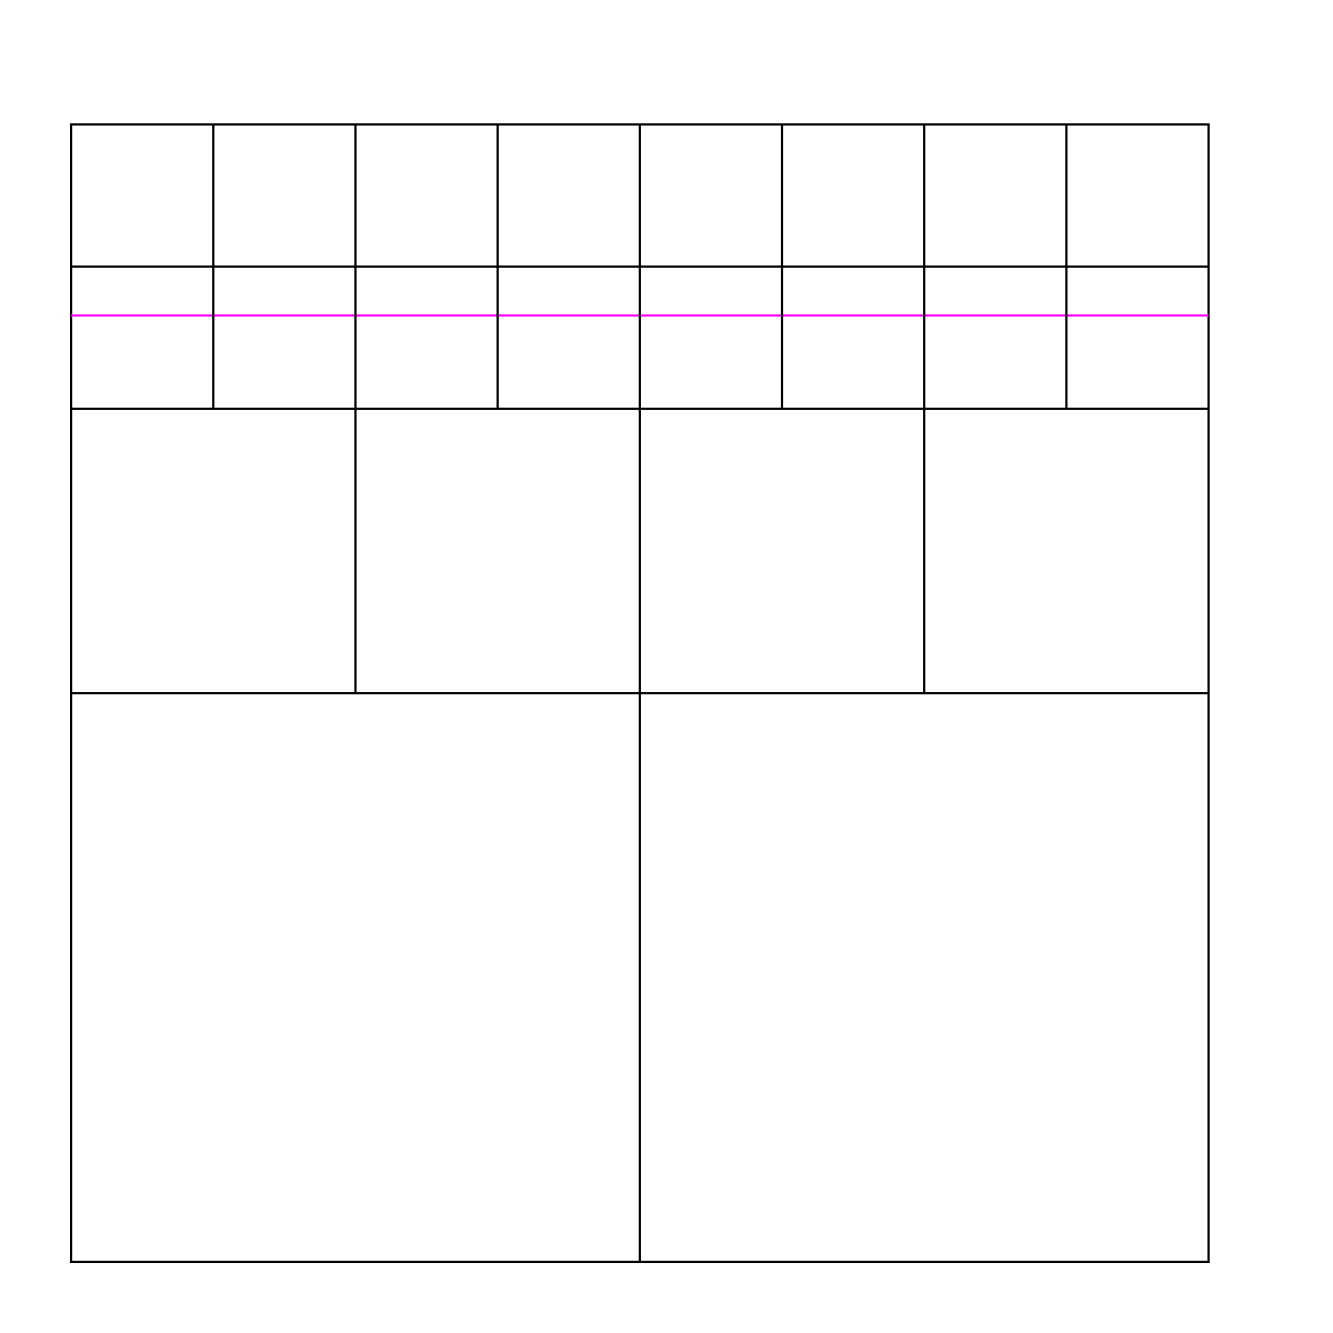
\includegraphics[width=4cm]{images/meshes/AMR/amr_3}\\
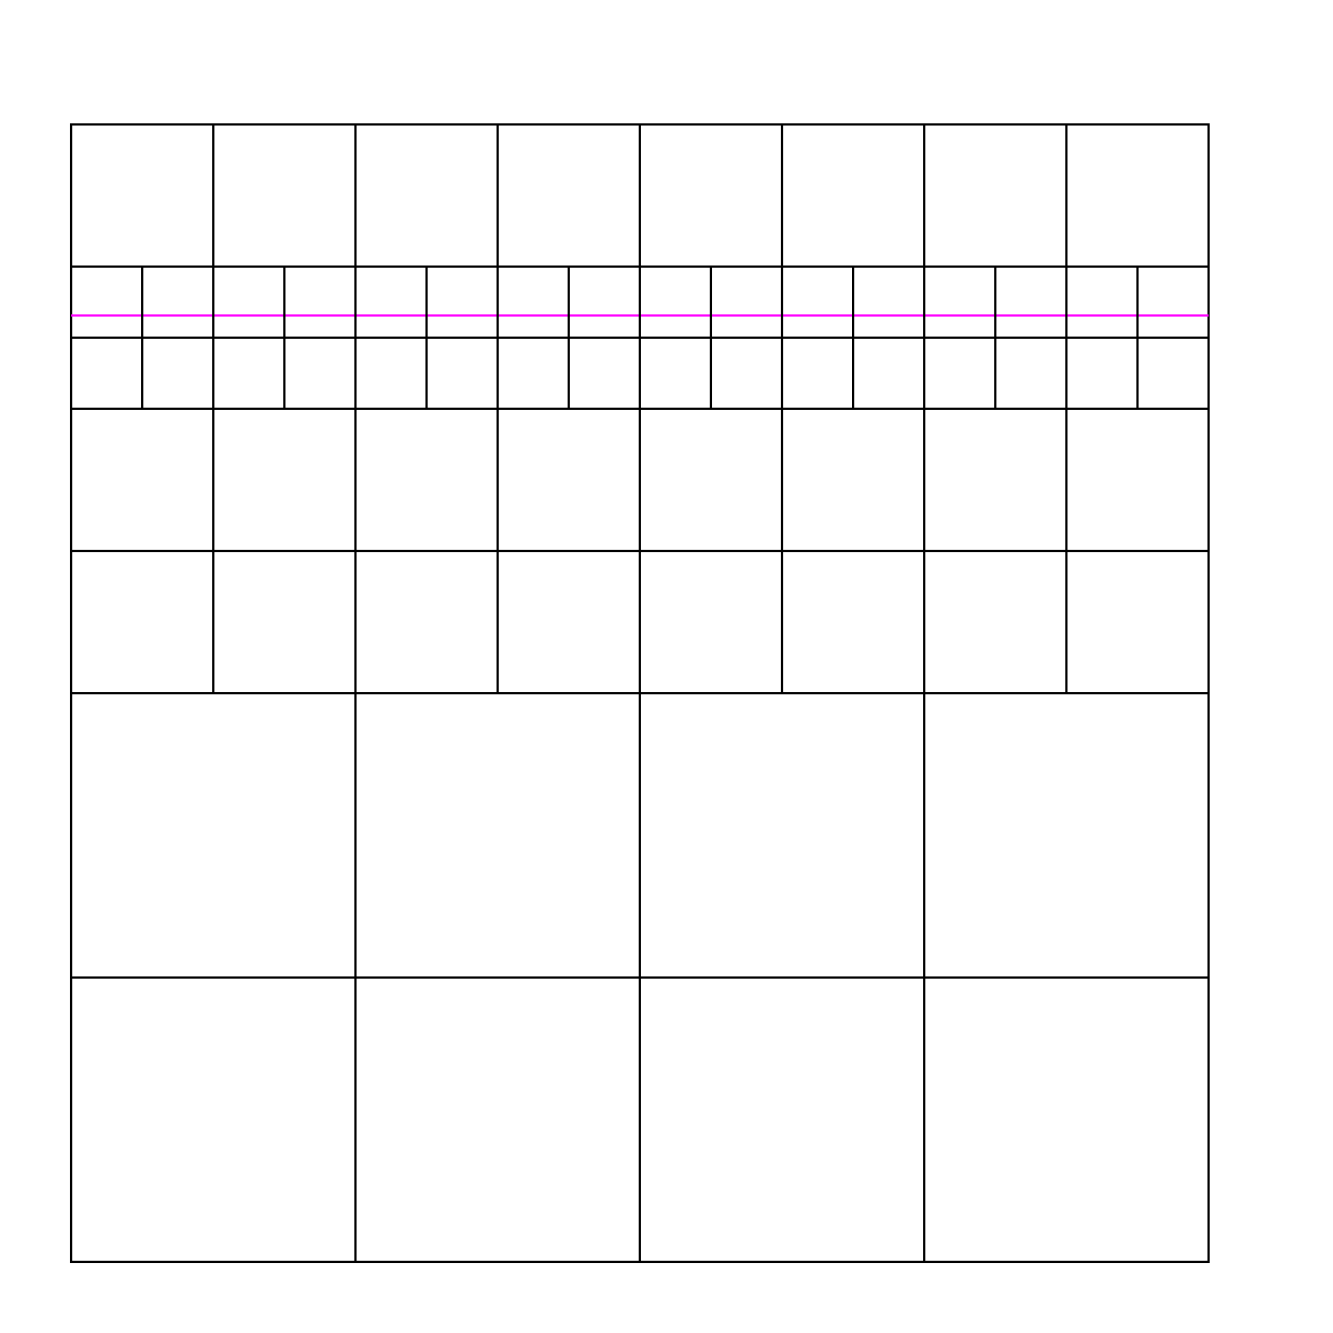
\includegraphics[width=4cm]{images/meshes/AMR/amr_4}
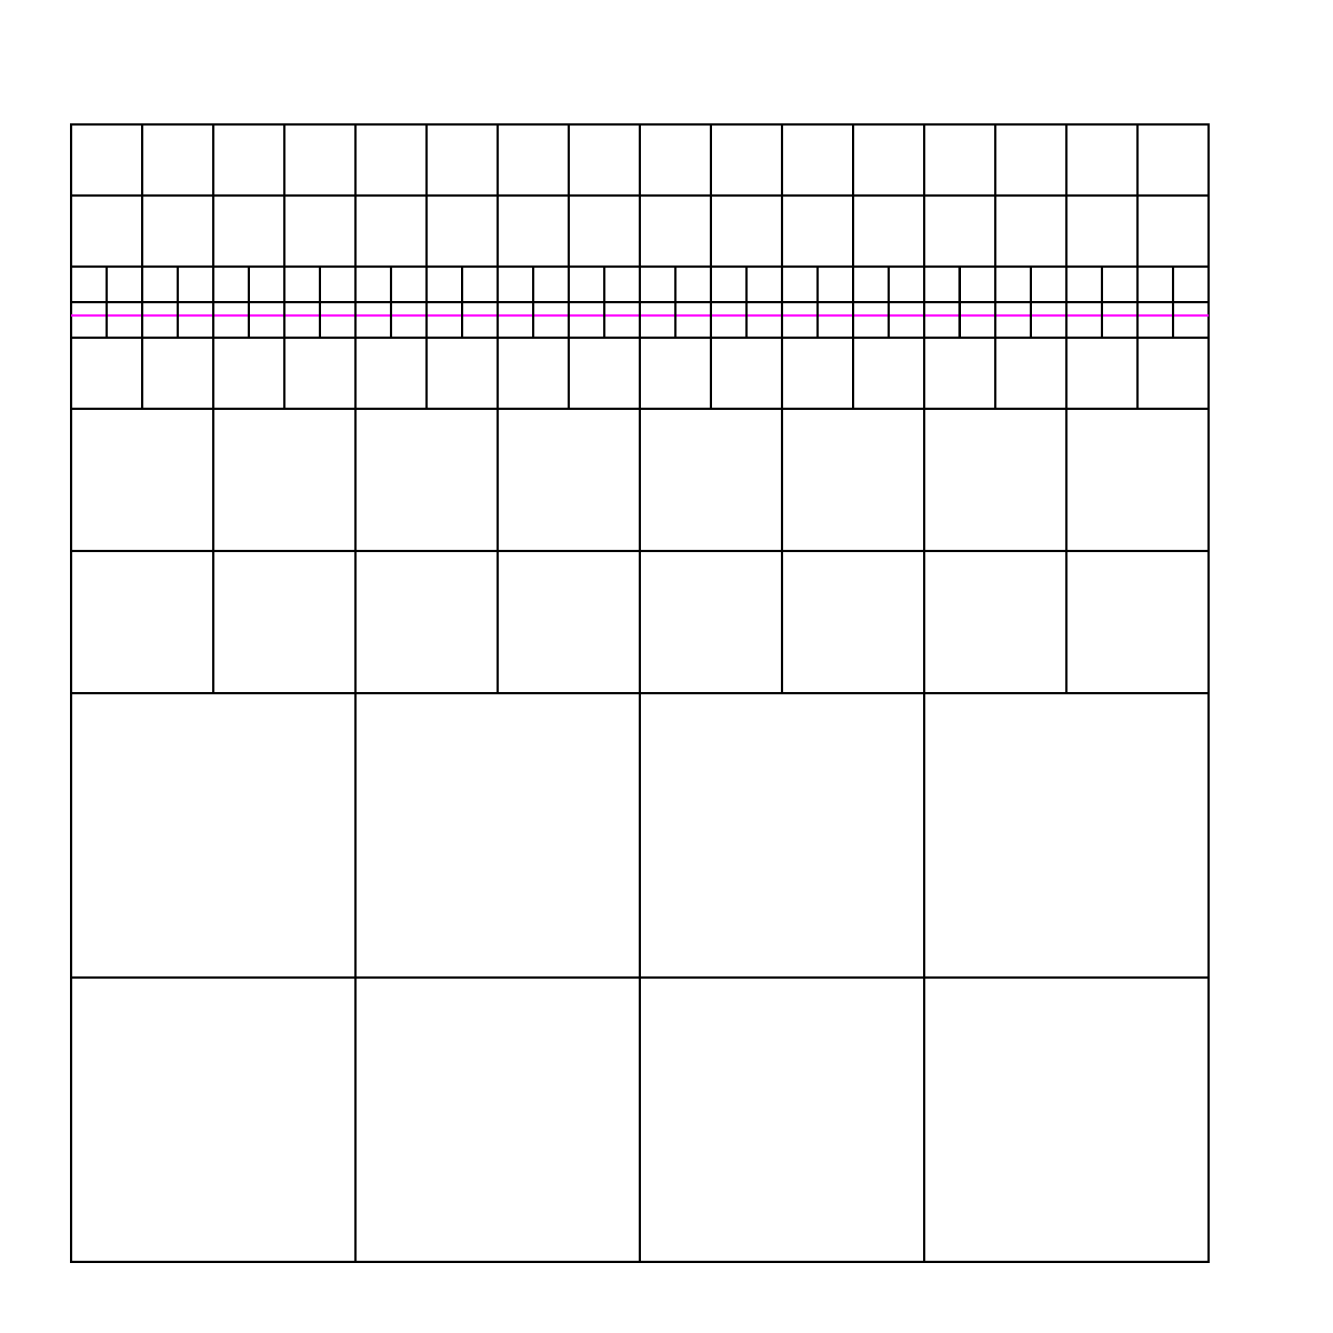
\includegraphics[width=4cm]{images/meshes/AMR/amr_5}
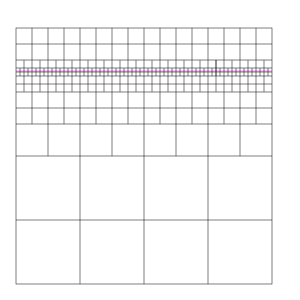
\includegraphics[width=4cm]{images/meshes/AMR/amr_6}
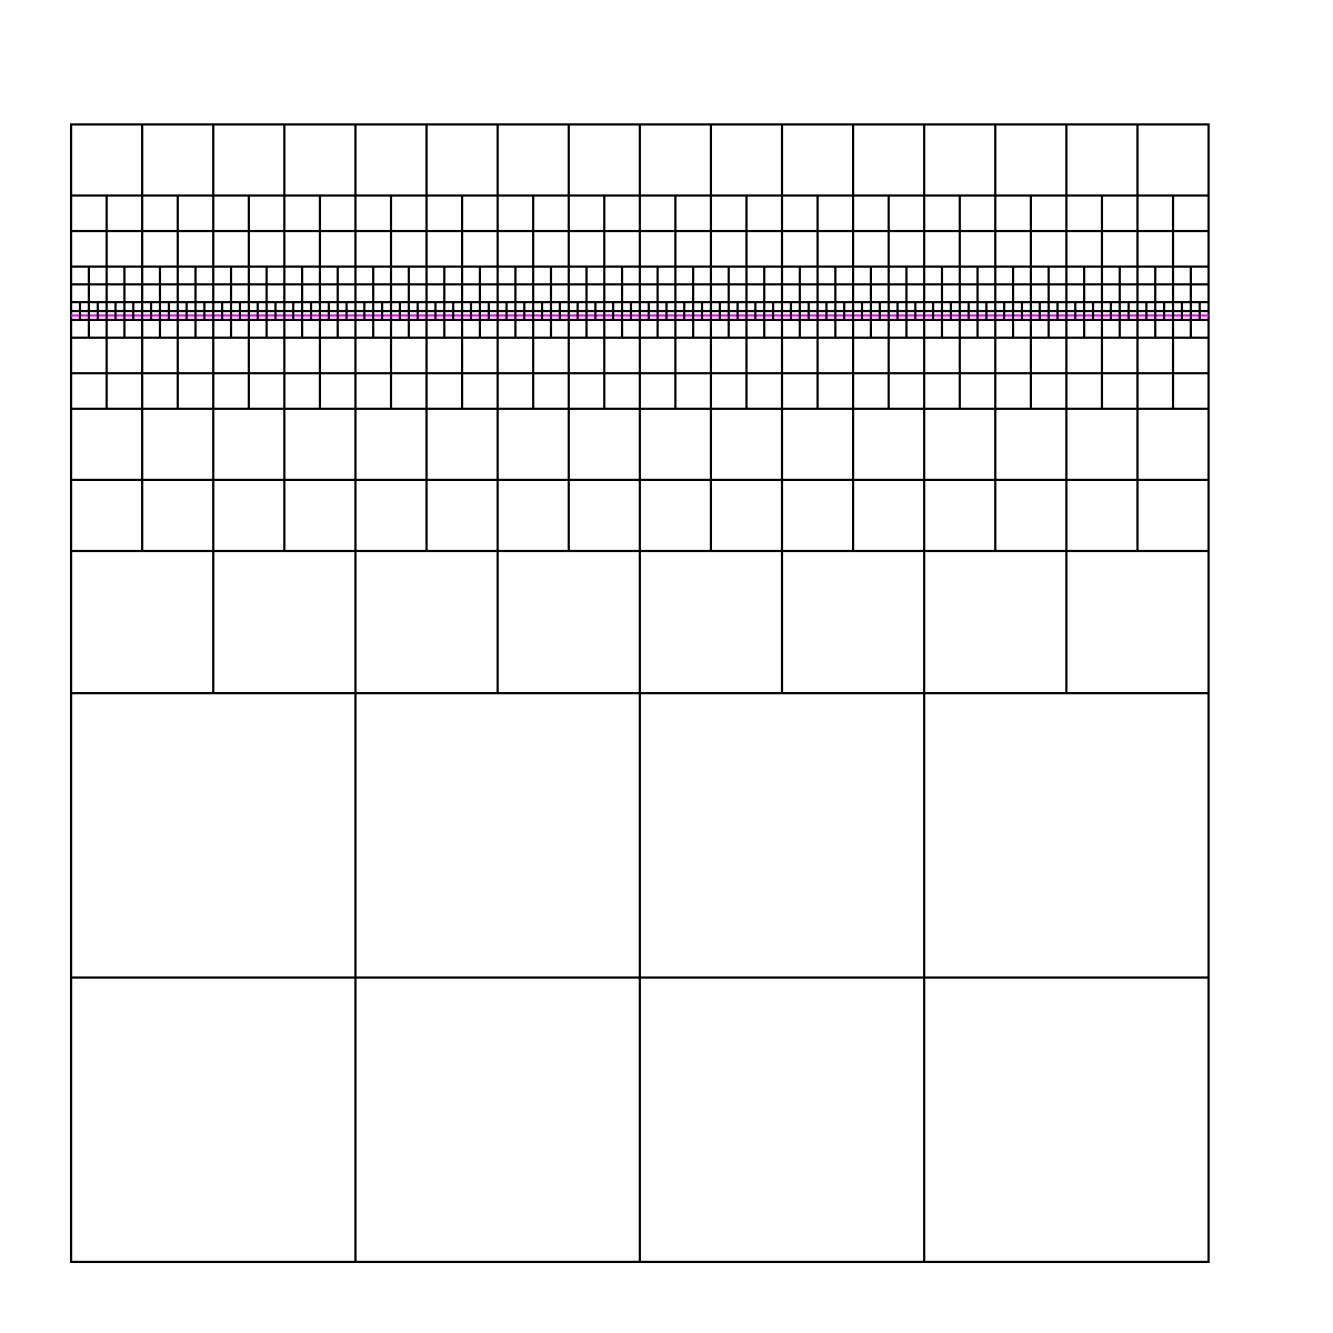
\includegraphics[width=4cm]{images/meshes/AMR/amr_7}


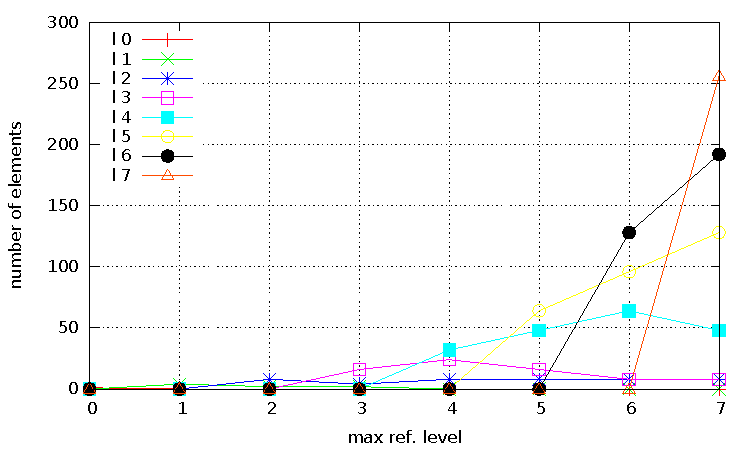
\includegraphics[width=5cm]{images/meshes/AMR/amr_data3.pdf}
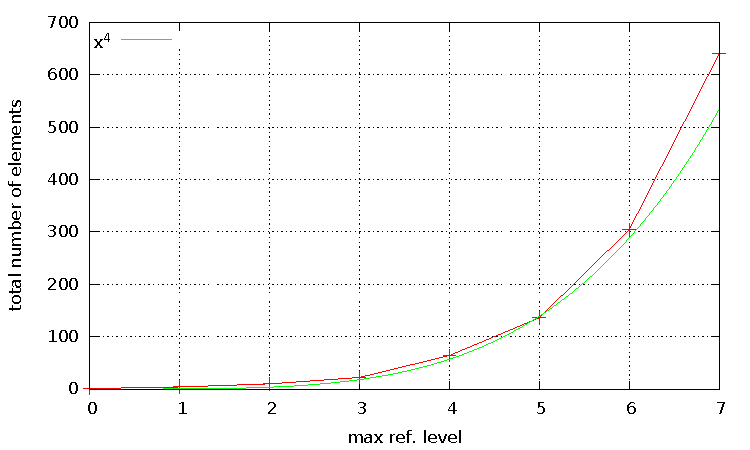
\includegraphics[width=5cm]{images/meshes/AMR/amr_data4.pdf}
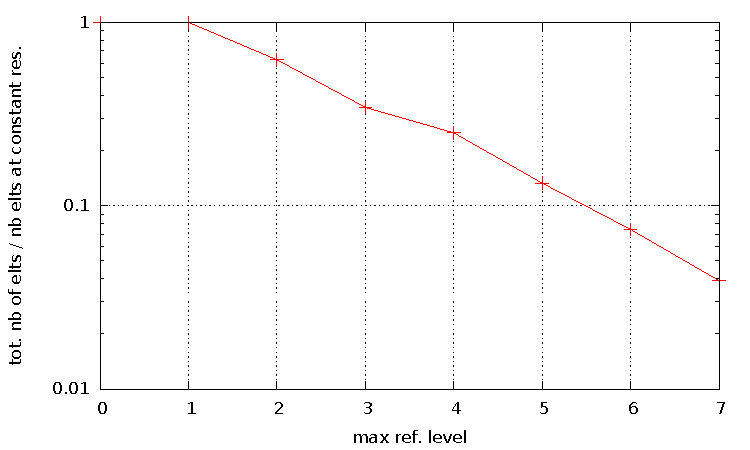
\includegraphics[width=5cm]{images/meshes/AMR/amr_data5.pdf}



